\documentclass[11pt,a4paper]{article}

\usepackage[utf8]{inputenc}
\usepackage[T1]{fontenc}
\usepackage[margin=2.5cm]{geometry}
\usepackage{amsmath,amssymb,amsthm}
\usepackage{booktabs,array}
\usepackage{enumitem}
\usepackage{tikz}
\usetikzlibrary{arrows.meta,calc,patterns,positioning}
\usepackage{pgfplots}
\pgfplotsset{compat=1.16}
\usepackage[most]{tcolorbox}
\tcbuselibrary{theorems,breakable,skins}
\usepackage[colorlinks=true,linkcolor=blue!50!black,urlcolor=blue!50!black]{hyperref}

% ---------- macros ----------
\newcommand{\R}{\mathbb{R}}
\newcommand{\dd}{\,\mathrm{d}}
\newcommand{\sr}{\emph{(slides\,?--?)}}
\newcommand{\Jc}{J_c}
\newcommand{\Jb}{\bar{J}_c}
\DeclareMathOperator{\rank}{rank}
\DeclareMathOperator{\blkdiag}{blkdiag}

% ---------- boxed theorem-like environments ----------
\newtcbtheorem[number within=section]{definition}{Definition}
  {enhanced,breakable,colback=gray!6,colframe=black!65,fonttitle=\bfseries,
   coltitle=white,colbacktitle=black!65,sharp corners,before upper={\parindent0pt}}{def}
\newtcbtheorem[use counter from=definition]{lemma}{Lemma}
  {enhanced,breakable,colback=green!4,colframe=green!40!black,fonttitle=\bfseries,
   coltitle=white,colbacktitle=green!40!black,sharp corners,before upper={\parindent0pt}}{lem}
\newtcbtheorem[use counter from=definition]{theorem}{Theorem}
  {enhanced,breakable,colback=red!4,colframe=red!55!black,fonttitle=\bfseries,
   coltitle=white,colbacktitle=red!55!black,sharp corners,before upper={\parindent0pt}}{thm}
\newtcbtheorem[use counter from=definition]{proposition}{Proposition}
  {enhanced,breakable,colback=orange!5,colframe=orange!60!black,fonttitle=\bfseries,
   coltitle=white,colbacktitle=orange!60!black,sharp corners,before upper={\parindent0pt}}{prop}
\newtcbtheorem[use counter from=definition]{corollary}{Corollary}
  {enhanced,breakable,colback=purple!4,colframe=purple!55!black,fonttitle=\bfseries,
   coltitle=white,colbacktitle=purple!55!black,sharp corners,before upper={\parindent0pt}}{cor}
\newtcbtheorem[use counter from=definition]{example}{Example}
  {enhanced,breakable,colback=yellow!8,colframe=yellow!40!black,fonttitle=\bfseries,
   coltitle=white,colbacktitle=yellow!40!black,sharp corners,before upper={\parindent0pt}}{ex}
\newtcbtheorem[use counter from=definition]{algorithm}{Algorithm}
  {enhanced,breakable,colback=cyan!4,colframe=cyan!45!black,fonttitle=\bfseries,
   coltitle=white,colbacktitle=cyan!45!black,sharp corners,before upper={\parindent0pt}}{alg}

\newtcolorbox{intuition}{enhanced,breakable,colback=blue!5,colframe=blue!60!black,
  title=Intuition,fonttitle=\bfseries,coltitle=white,colbacktitle=blue!60!black,
  sharp corners,before upper={\parindent0pt}}

\newcommand{\photoph}[2]{%
  \begin{center}\fbox{\parbox{0.8\linewidth}{\centering\vspace{1.3cm}%
  \textbf{PHOTO PLACEHOLDER}\\[2pt] #1\\[2pt] \emph{Pick it from slide #2}\vspace{1.3cm}}}\end{center}}

\title{\textbf{Contact Constraints}\\[2pt]
\large From Geometric Conditions to Constrained Dynamics\\[2pt]
\normalsize Agile and Legged Robots module --- Elective in Robotics\\
AI and Robotics (M.Sc.), Sapienza University of Rome --- Prof.\ Lanari}
\author{Lecture notes}
\date{}

\begin{document}
\maketitle

\begin{tcolorbox}[colback=yellow!10,colframe=yellow!50!black,title=Read me first,fonttitle=\bfseries,sharp corners]
These notes were written \emph{without} the slide deck and without a companion PDF.
Section titles follow the standard logical order of the topic (holonomic constraints and tangent space
$\to$ floating-base dynamics $\to$ geometry of contact
$\to$ kinematic constraints $\to$ constrained dynamics $\to$ friction $\to$ control),
\emph{not} verbatim slide titles, and every slide range is a placeholder
\sr\ to be filled in once the deck is at hand. The same holds for the photo placeholders.
All figures are original TikZ/pgfplots drawings.
\end{tcolorbox}

\tableofcontents
\newpage

% =====================================================================
\section{Holonomic Constraints \sr}

\subsection{Constraints on the configuration \sr}

Let $q\in\mathcal Q$ be the generalized coordinates (locally $q\in\R^{n_q}$). A mechanical
constraint restricts which configurations, and hence which motions, the system can have.

\begin{definition}{Holonomic constraint}{holo}
A \emph{holonomic constraint} is a smooth equation on the configuration only,
\begin{equation}\label{eq:holo}
  \varphi(q)=0,\qquad \varphi:\mathcal Q\to\R^{m},
\end{equation}
with $m$ independent scalar equations. The set of feasible configurations is
$\mathcal C=\{q:\varphi(q)=0\}$. A constraint on velocities $A(q)\dot q=0$ that cannot be
integrated into the form \eqref{eq:holo} is \emph{nonholonomic} (e.g.\ a wheel rolling
without slipping).
\end{definition}

\begin{proposition}{The constraint manifold}{cman}
Let $J(q)=\partial\varphi/\partial q$. If $J(q)$ has full row rank $m$ on $\mathcal C$
(a \emph{regular} constraint), then $\mathcal C$ is a smooth embedded submanifold of
$\mathcal Q$ of dimension $n_q-m$.
\end{proposition}

\begin{intuition}
Each independent equation removes one degree of freedom. A bead on a wire in 3D has
$3-2=1$ degree of freedom (two equations pin it to the wire); a point on a sphere has
$3-1=2$. In legged robotics, the stance foot is the bead and the leg is the wire: gluing the
foot to the floor removes $3$ degrees of freedom from the robot.
\end{intuition}

\begin{example}{Constraints that appear in legged robots}{holoex}
\begin{itemize}[nosep]
  \item \textbf{Fixed stance foot (no slip):} $\varphi(q)=p_c(q)-p_c^{0}=0$, $m=3$ for a point
        contact (the foot position equals a constant).
  \item \textbf{Flat foot that cannot rotate:} position and orientation fixed, $m=6$.
  \item \textbf{Closed kinematic chain} (e.g.\ a parallel leg or two hands on one object):
        $\varphi(q)=p_A(q)-p_B(q)=0$.
\end{itemize}
\end{example}

\subsection{Admissible velocities: the tangent space \sr}

Which velocities are compatible with staying on $\mathcal C$?

\begin{definition}{Tangent space of the constraint manifold}{tan}
The \emph{tangent space} to $\mathcal C$ at $q\in\mathcal C$ is the set of velocities of
all smooth curves lying in $\mathcal C$ and passing through $q$,
\[
  T_q\mathcal C=\big\{\dot\gamma(0)\;:\;\gamma:(-\varepsilon,\varepsilon)\to\mathcal C
  \ \text{smooth},\ \gamma(0)=q\big\}.
\]
Its elements are called \emph{admissible} (or \emph{virtual}) velocities.
\end{definition}

\begin{theorem}{Admissible velocities are the kernel of the Jacobian}{tan}
If $J(q)$ has full row rank $m$, then
\begin{equation}\label{eq:tan}
  T_q\mathcal C=\ker J(q)=\{v:\ J(q)\,v=0\},\qquad \dim T_q\mathcal C=n_q-m .
\end{equation}
\end{theorem}
\begin{proof}
($\subseteq$) If $\gamma$ lies in $\mathcal C$ then $\varphi(\gamma(t))=0$ for all $t$;
differentiating at $t=0$ gives $J(q)\dot\gamma(0)=0$.

($\supseteq$) Since $\rank J=m$, reorder the coordinates $q=(q_a,q_b)$, $q_b\in\R^m$, so that
$J_b=\partial\varphi/\partial q_b$ is invertible. By the implicit function theorem there is a
smooth $g$ with $\varphi(q_a,g(q_a))=0$ near $q$, and $\mathrm Dg=-J_b^{-1}J_a$. For
$v=(v_a,v_b)\in\ker J$ we have $J_a v_a+J_b v_b=0$, i.e.\ $v_b=\mathrm Dg\,v_a$. The curve
$\gamma(t)=\big(q_a+t v_a,\;g(q_a+t v_a)\big)$ lies in $\mathcal C$ and has $\dot\gamma(0)=v$.
The dimension follows from rank--nullity.
\end{proof}

\begin{intuition}
The gradient of each constraint, a row of $J$, points \emph{across} the constraint surface.
A velocity is admissible when it has no component across it, that is, when it is
\emph{tangent}. Number: a point on the unit circle, $\varphi(x,y)=x^2+y^2-1$, at
$q=(1,0)$ has $J=[2x\ \ 2y]=[2\ \ 0]$, so $\ker J=\operatorname{span}\{(0,1)\}$: the point can
only move vertically (tangent to the circle), exactly as expected.
\end{intuition}

\begin{figure}[ht]
\centering
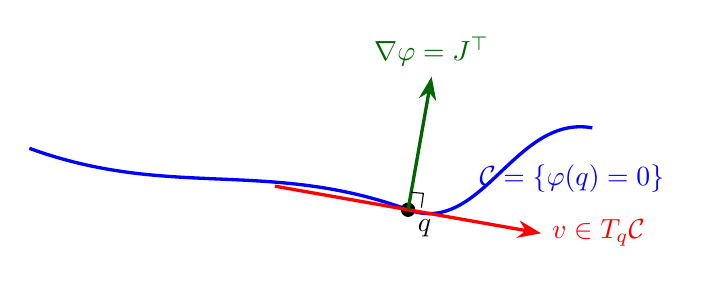
\begin{tikzpicture}[>=Stealth,scale=1.3]
  \draw[very thick,blue] (-0.3,2.2) to[out=-20,in=160] (3.4,1.6) to[out=-20,in=170] (5.2,2.4);
  \node[blue] at (5.0,1.9) {$\mathcal C=\{\varphi(q)=0\}$};
  \def\px{3.4}\def\py{1.6}
  \fill (\px,\py) circle (2pt) node[below right] {$q$};
  \draw[->,very thick,red] (\px-1.3,\py+0.23) -- (\px+1.3,\py-0.23) node[right] {$v\in T_q\mathcal C$};
  \draw[->,very thick,green!40!black] (\px,\py) -- (\px+0.23,\py+1.3) node[above] {$\nabla\varphi=J^\top$};
  \draw (\px+0.13,\py+0.02) -- (\px+0.15,\py+0.16) -- (\px+0.03,\py+0.17);
\end{tikzpicture}
\caption{At $q$ the admissible velocities form the tangent line $\ker J$; the rows of $J$ (gradients of $\varphi$) are orthogonal to it.}
\end{figure}

\begin{corollary}{Floating base and manifold-valued coordinates}{fbtan}
When $q$ contains a rotation (floating base, $SE(3)$) one uses the generalized velocity
$v$ with $\dot q=E(q)v$ and the Jacobian $J_v(q)=\frac{\partial\varphi}{\partial q}E(q)$, so that
$\dot\varphi=J_v(q)v$. Then \eqref{eq:tan} holds with $v\in\ker J_v$ and dimension
$n_v-m$ (we write $J$ for $J_v$ from now on).
\end{corollary}

\begin{proposition}{Parametrization of admissible velocities}{par}
Let $Z(q)\in\R^{n_v\times(n_v-m)}$ have columns forming a basis of $\ker J(q)$ (obtained
e.g.\ from a QR/SVD of $J^\top$). Then every admissible velocity is $v=Z(q)\,\nu$ for a unique
$\nu\in\R^{n_v-m}$.
\end{proposition}

\begin{intuition}
The vector $\nu$ plays the role of the velocities of an \emph{equivalent unconstrained
robot} with fewer degrees of freedom. Number: a quadruped with $n_v=18$ and four fixed point
feet has $m=12$, hence $\nu\in\R^{6}$; with a single fixed point foot, $m=3$ and $\nu\in\R^{15}$.
The projector $N=I-\Jb\Jc$ of Section~\ref{sec:cdyn} is one explicit choice of such a basis map.
\end{intuition}

\begin{example}{Planar pendulum: point mass on a circle in Cartesian coordinates}{pendcart}
Consider a planar pendulum consisting of a point mass $m_p$ attached to a rigid, massless rod of length $l$ pivoted at the origin $(0,0)$. Instead of using the minimal angular coordinate $\theta$, we describe the system in redundant Cartesian coordinates of the mass:
\[
  q = \begin{bmatrix} x \\ y \end{bmatrix} \in \R^2 \qquad (n_q = 2).
\]

\textbf{1. Holonomic constraint and manifold:}\\
The rigid link maintains a fixed distance $l$ from the pivot, yielding the geometric constraint:
\[
  \varphi(q) = \frac{1}{2}\big(x^2 + y^2 - l^2\big) = 0 \qquad (m = 1).
\]
The constraint manifold $\mathcal C = \{q \in \R^2 : \|q\| = l\}$ is a 1-dimensional circle ($S^1$) embedded in $\R^2$. The constraint Jacobian is:
\[
  J(q) = \frac{\partial \varphi}{\partial q} = \begin{bmatrix} x & y \end{bmatrix} = q^\top \in \R^{1 \times 2}.
\]
Since $l > 0$, the mass cannot be at the origin on $\mathcal C$, so $\rank J(q) = 1$ everywhere. Thus $\dim T_q\mathcal C = n_q - m = 2 - 1 = 1$. The gradient row $J(q)^\top = q$ points radially outward, perpendicular to the circle.

\smallskip
\textbf{2. Tangent space and admissible velocities:}\\
By Theorem~\ref{thm:tan}, a generalized velocity $v = \dot q = [\dot x\ \ \dot y]^\top$ is admissible ($v \in T_q\mathcal C$) if and only if:
\[
  J(q)\,v = 0 \iff x\dot x + y\dot y = q^\top \dot q = 0.
\]
Geometrically, the velocity must be orthogonal to the position vector $q$, ensuring that motion remains purely tangential to the circle.

\smallskip
\textbf{3. Null-space basis and velocity parametrization:}\\
Since $\dim\ker J(q) = 1$, we can choose a basis matrix $Z(q) \in \R^{2 \times 1}$ for $\ker J(q)$:
\[
  Z(q) = \begin{bmatrix} -y \\ x \end{bmatrix}, \qquad \text{satisfying } J(q)Z(q) = x(-y) + y(x) = 0.
\]
By Proposition~\ref{prop:par}, every admissible velocity is uniquely represented by a scalar quasi-velocity $\nu \in \R$:
\[
  v = \begin{bmatrix} \dot x \\ \dot y \end{bmatrix} = Z(q)\,\nu = \begin{bmatrix} -y \\ x \end{bmatrix}\nu.
\]

\smallskip
\textbf{4. Equivalence with minimal coordinate $\theta$:}\\
Parameterizing the circle with the angle $\theta$ measured counterclockwise from the downward vertical:
\[
  x = l\sin\theta, \qquad y = -l\cos\theta.
\]
Differentiating with respect to time yields:
\[
  v = \begin{bmatrix} \dot x \\ \dot y \end{bmatrix} = \begin{bmatrix} l\cos\theta \\ l\sin\theta \end{bmatrix}\dot\theta = \begin{bmatrix} -y \\ x \end{bmatrix}\dot\theta.
\]
Comparing with $v = Z(q)\nu$, we find $\nu = \dot\theta$. The scalar $\nu$ is exactly the angular velocity of the equivalent unconstrained 1-DOF system.

\smallskip
\textbf{5. Constraint forces and accelerations (preview):}\\
Differentiating $J(q)v = 0$ yields the admissible acceleration condition:
\[
  J(q)\dot v + \dot J(q,v)v = 0 \implies x\ddot x + y\ddot y + (\dot x^2 + \dot y^2) = 0 \implies q^\top \ddot q = -\|v\|^2 = -l^2\dot\theta^2.
\]
This specifies the inward centripetal acceleration required to stay on the circle. The constraint force that enforces this motion is:
\[
  F_{\mathrm{con}} = J(q)^\top \lambda = \lambda \begin{bmatrix} x \\ y \end{bmatrix},
\]
which is the tension along the rod. Since $F_{\mathrm{con}}^\top v = \lambda q^\top \dot q = 0$, the constraint force does zero virtual work on any admissible velocity.

\begin{center}
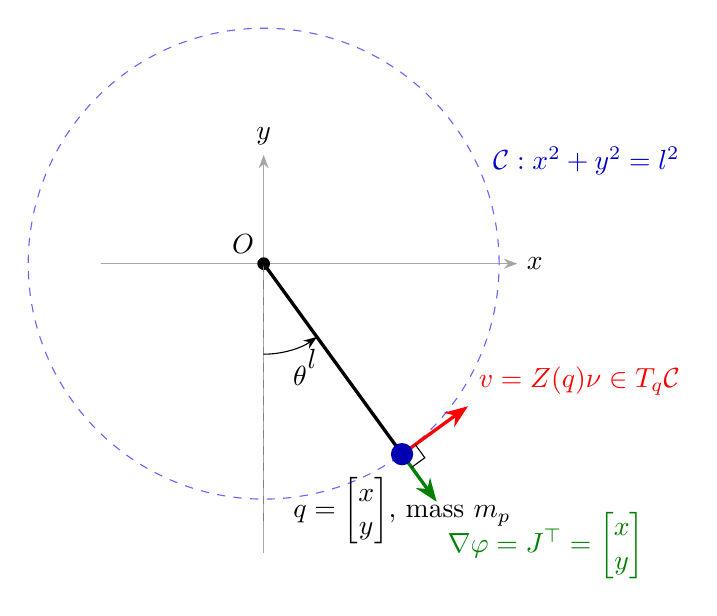
\begin{tikzpicture}[>=Stealth,scale=1.15]
  % Axes
  \draw[->,thin,gray!70] (-1.8,0) -- (2.8,0) node[right,black] {$x$};
  \draw[->,thin,gray!70] (0,-3.2) -- (0,1.2) node[above,black] {$y$};
  \fill (0,0) circle (2pt) node[above left] {$O$};

  \def\len{2.6}
  \def\ang{36}

  % Trajectory circle
  \draw[dashed,blue!60] (0,0) circle (\len);
  \node[blue!80!black,right] at ({1.03*\len*cos(25)},{1.03*\len*sin(25)}) {$\mathcal C: x^2+y^2=l^2$};

  % Reference vertical line for theta
  \draw[dashed,gray] (0,0) -- (0,-2.9);
  \draw[->] (0,-1.0) arc (-90:{-90+\ang}:1.0);
  \node at ({1.3*sin(\ang/2)},{-1.3*cos(\ang/2)}) {$\theta$};

  % Mass point
  \coordinate (M) at ({\len*sin(\ang)},{-\len*cos(\ang)});

  % Pendulum rod
  \draw[very thick] (0,0) -- (M) node[midway,left=2pt] {$l$};

  % Normal gradient vector J^T
  \draw[->,very thick,green!50!black] (M) -- ($ (M) + 0.65*({sin(\ang)},{-cos(\ang)}) $)
    node[below right] {$\nabla\varphi = J^\top = \begin{bmatrix} x \\ y \end{bmatrix}$};

  % Tangent velocity vector v
  \draw[->,very thick,red] (M) -- ($ (M) + 0.9*({cos(\ang)},{sin(\ang)}) $)
    node[above right] {$v = Z(q)\nu \in T_q\mathcal C$};

  % Right angle mark
  \draw ($ (M) + 0.18*({sin(\ang)},{-cos(\ang)}) $) --
        ($ (M) + 0.18*({sin(\ang)},{-cos(\ang)}) + 0.18*({cos(\ang)},{sin(\ang)}) $) --
        ($ (M) + 0.18*({cos(\ang)},{sin(\ang)}) $);

  % Mass bob
  \fill[blue!70!black] (M) circle (3.5pt) node[below=5pt,black] {$q = \begin{bmatrix} x \\ y \end{bmatrix}$, mass $m_p$};
\end{tikzpicture}
\end{center}
\end{example}

\subsection{Constraint forces and admissible accelerations \sr}

\begin{proposition}{Constraint forces do no work}{work}
The range of $J^\top$ is the orthogonal complement of $\ker J$. Hence any generalized force
of the form $F_{\mathrm{con}}=J(q)^\top\lambda$, with $\lambda\in\R^m$ (the \emph{Lagrange
multipliers}), has zero power on admissible velocities:
$F_{\mathrm{con}}^\top v=\lambda^\top J v=0$ for all $v\in T_q\mathcal C$.
\end{proposition}

\begin{intuition}
An ideal wire pushes the bead \emph{perpendicular} to the wire: it can bend its path but
cannot speed it up or slow it down. The same holds for $\Jc^\top f_c$ in \eqref{eq:eom}:
a sticking foot supplies forces that never do work, because the foot does not move. This is
d'Alembert's principle and is the reason the contact forces will be eliminated by projecting
onto $\ker\Jc$ later on.
\end{intuition}

\begin{proposition}{Admissible accelerations}{accadm}
Along a trajectory staying in $\mathcal C$, $\varphi(q(t))\equiv0$ implies
$J v=0$ and
\begin{equation}\label{eq:accholo}
  J(q)\,\dot v+\dot J(q,v)\,v=0 .
\end{equation}
Admissible accelerations therefore form an \emph{affine} subspace parallel to $\ker J$,
not $\ker J$ itself.
\end{proposition}

\begin{intuition}
Moving tangentially is not enough: the path of the point must also \emph{bend} to follow
the constraint, and bending requires an acceleration across the surface. Check with the
circle: at $q=(1,0)$ with $v=(0,1)$, $\dot J v=2\dot x\,v_x+2\dot y\,v_y=2$, so
\eqref{eq:accholo} gives $2a_x+2=0$, i.e.\ $a_x=-1=-v^2/r$: the centripetal acceleration.
\end{intuition}

\begin{definition}{Unilateral constraint and tangent cone}{cone0}
A \emph{unilateral} (inequality) constraint $\varphi(q)\ge0$ allows leaving the boundary.
When it is active ($\varphi=0$) the admissible velocities are no longer a subspace but the
half-space (more generally a cone) $\{v:\ J(q)v\ge0\}$.
\end{definition}

\begin{intuition}
A foot lying on the ground may rotate and lift off but cannot move into the floor, so the
set of allowed velocities is a half-space. It becomes the subspace $\ker J$ only when the
foot is sticking. Section~\ref{sec:geom} turns this into the Signorini conditions.
\end{intuition}

% =====================================================================
\section{Floating-Base Dynamics \sr}\label{sec:fb}

\subsection*{Why contacts matter \sr}
A legged (or humanoid) robot is a \emph{floating-base} system: no joint connects it to the
world, so it moves only by pushing against the environment. Contacts are therefore not a
disturbance to be rejected: they are the \emph{only} way the robot can accelerate its
centre of mass. Modelling them correctly means answering three questions:
\begin{enumerate}[nosep]
  \item \textbf{Geometry:} when is a foot touching the ground?
  \item \textbf{Kinematics:} what does ``touching'' imply on velocities and accelerations?
  \item \textbf{Dynamics and forces:} which forces can the ground exert, and how do they enter the equations of motion?
\end{enumerate}


\begin{figure}[ht]
\centering
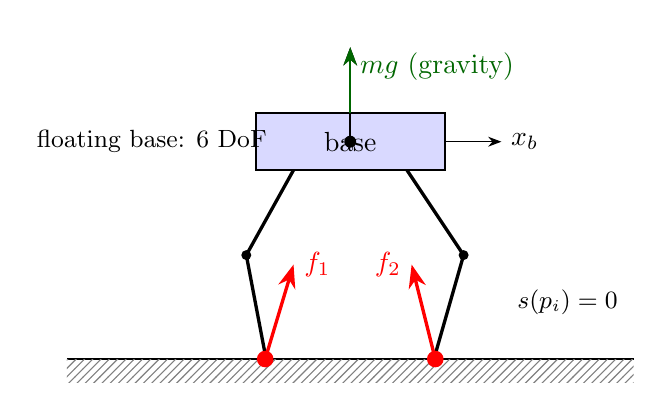
\begin{tikzpicture}[scale=1.2,>=Stealth]
  % ground
  \draw[thick] (-3,0) -- (3,0);
  \fill[pattern=north east lines,pattern color=gray] (-3,-0.25) rectangle (3,0);
  % base
  \draw[fill=blue!15,thick] (-1,2) rectangle (1,2.6);
  \node at (0,2.3) {base};
  % legs
  \draw[very thick] (-0.6,2) -- (-1.1,1.1) -- (-0.9,0.05);
  \draw[very thick] (0.6,2) -- (1.2,1.1) -- (0.9,0.05);
  \fill (-1.1,1.1) circle (1.5pt) (1.2,1.1) circle (1.5pt);
  % feet
  \fill[red] (-0.9,0) circle (2.5pt) (0.9,0) circle (2.5pt);
  % contact forces
  \draw[->,red,very thick] (-0.9,0) -- (-0.6,1.0) node[right] {$f_1$};
  \draw[->,red,very thick] (0.9,0) -- (0.65,1.0) node[left] {$f_2$};
  % CoM + gravity
  \fill[black] (0,2.3) circle (1.8pt);
  \draw[->,thick] (0,2.3) -- (0,3.3) node[above] {};
  \draw[->,thick,green!40!black] (0,2.6) -- (0,3.3);
  \node[green!40!black,right] at (0,3.1) {$mg$ (gravity)};
  % base frame
  \draw[->] (1,2.3) -- (1.6,2.3) node[right] {$x_b$};
  \node at (-2.1,2.3) {\small floating base: 6 DoF};
  \node at (2.3,0.6) {\small $s(p_i)=0$};
\end{tikzpicture}
\caption{A floating-base biped in double support. The ground forces $f_1,f_2$ (red) are the only external actions besides gravity.}
\end{figure}

\begin{intuition}
Think of swimming versus walking. A swimmer pushes water and the water pushes back; a
walker does exactly the same with the ground. If the ground cannot push back (ice, air,
flight phase), the centre of mass follows a ballistic trajectory and no joint torque can
change it. Everything that follows is about making ``the ground pushes back'' precise.
\end{intuition}


Let $n$ be the number of actuated joints. The configuration is $q=(q_b,q_j)$ with
$q_b\in SE(3)$ the base pose and $q_j\in\R^n$ the joint angles. The generalized velocity is
$v=(v_b,\dot q_j)\in\R^{n_v}$, $n_v=n+6$, with $v_b\in\R^6$ the base twist.

\begin{definition}{Floating-base equations of motion}{fb}
\begin{equation}\label{eq:eom}
  M(q)\,\dot v + h(q,v) \;=\; S^{\top}\tau \;+\; \sum_{i=1}^{k} J_i(q)^{\top} f_i
  \;=\; S^{\top}\tau + \Jc(q)^{\top} f_c ,
\end{equation}
where $M\succ0$ is the inertia matrix, $h$ collects Coriolis, centrifugal and gravity terms,
$S=[\,0_{n\times 6}\;\; I_n\,]$ is the actuation selection matrix, $\tau\in\R^n$ the joint
torques, $f_i$ the force at the $i$-th contact point, $J_i=\partial p_i/\partial q$ the
(velocity) Jacobian of that point, and $\Jc=[J_1;\dots;J_k]$, $f_c=[f_1;\dots;f_k]$.
\end{definition}

\begin{intuition}
The term $\Jc^\top f_c$ is just the principle of virtual work: a force $f_i$ applied at a
point is mapped into generalized forces through the transpose of the point's Jacobian.
The matrix $S^\top$ says that torques act only on the last $n$ rows: \emph{nothing pushes
directly on the base}. Count for a quadruped with $n=12$: $n_v=18$ equations, $12$ torques
to act with, so the six base rows are driven \emph{only} by contact forces.
\end{intuition}

% =====================================================================
\section{Contact: Geometric Conditions \sr}\label{sec:geom}

\subsection{Why a gap function $d$ and not an equality constraint $h(q)=0$? \sr}

A fundamental question arises when transitioning from textbook analytical mechanics to contact mechanics in robotics: \emph{why can we not simply model contact with the ground using an equality constraint $h(q)=0$?}

\begin{proposition}{Bilateral constraint $h(q)=0$ vs.\ unilateral gap $d(q)\ge 0$}{gap_vs_h}
\begin{itemize}[nosep]
  \item \textbf{Equality constraint $h(q)=0$ (bilateral):}
  Enforces $h(q(t))\equiv 0$ identically for all times. The associated Lagrange multiplier $\lambda \in \R$ is sign-unconstrained (can be positive or negative, pushing or pulling). This models a bilateral mechanical joint (e.g.\ a weld, pin, or bead on a wire), effectively ``gluing'' the foot to the ground. It \emph{cannot} represent detachment, flight phases, or gait switching.
  \item \textbf{Gap function $d(q)\ge 0$ (unilateral):}
  Contact with the environment is a physical barrier that restricts motion in only one direction. The distance (or signed gap) $d(q) = n^\top(p(q)-p_{\text{surf}}) \ge 0$ is an \emph{inequality} constraint. The ground can only push ($\lambda_n \ge 0$), never pull. Contact is intermittent: when $d(q)>0$, the foot is in the air and $\lambda_n=0$; when $d(q)=0$, contact is active and $\lambda_n\ge 0$.
\end{itemize}
\end{proposition}

\begin{table}[ht]
\centering
\small
\renewcommand{\arraystretch}{1.25}
\begin{tabular}{@{}p{3.5cm}p{5.5cm}p{5.5cm}@{}}
\toprule
\textbf{Property} & \textbf{Equality Constraint $h(q)=0$} & \textbf{Unilateral Gap $d(q)\ge 0$} \\
\midrule
Nature & Bilateral (two-sided, permanent) & Unilateral (one-sided, intermittent) \\
Reaction force & Sign-unconstrained ($\lambda \in \R$, push or pull) & Unidirectional ($\lambda_n \ge 0$, push only) \\
Liftoff / Detachment & Impossible ($h(q)\equiv 0$ forever) & Allowed ($d(q) > 0 \implies \lambda_n = 0$) \\
Physical analogue & Welded joint, slider rail, bilateral guide & Rigid ground, obstacle, non-sticky surface \\
Mathematical form & Differential-Algebraic Equations (DAEs) & Complementarity / Non-smooth hybrid system \\
\bottomrule
\end{tabular}
\caption{Comparison: classical bilateral equality constraint $h(q)=0$ versus unilateral contact gap $d(q)\ge 0$.}
\label{tab:gap_vs_h}
\end{table}

\begin{intuition}
If contact were modeled by $h(q)=p_z(q)=0$, the robot's feet would be bolted to the floor. Any attempt to lift a leg would produce an infinite or negative downward holding force $\lambda_z < 0$, making jumping, walking, or running physically impossible. Legged robots achieve locomotion precisely by breaking and making contact with the environment, requiring the unilateral gap formulation.
\end{intuition}

\subsection{The signed gap function and Signorini conditions \sr}

\begin{definition}{Signed gap function and contact condition}{gap}
For a candidate contact point $p_i(q)$ and a surface with outward unit normal $n$, the
\emph{signed gap function} $s(p)$ (often also denoted $d(q)$) is defined as
\begin{equation}\label{eq:signed_gap}
  s(p_i) = n^{\top}\big(p_i(q)-p_{\text{surf}}\big).
\end{equation}
For flat ground with $n=e_z$ and $p_{\text{surf},z}=0$, this is simply the vertical elevation:
$s(p_i)=p_{i,z}(q)$.
The geometric contact states are:
\begin{itemize}[nosep]
  \item $s(p_i) > 0$: no contact (flight/swing phase, foot in the air);
  \item $s(p_i) = 0$: contact is \emph{active} (foot touching the surface);
  \item $s(p_i) < 0$: interpenetration (physically inadmissible).
\end{itemize}
Non-penetration therefore requires $s(p_i) \ge 0$ (or $d(q) \ge 0$).
\end{definition}

The normal contact force $\lambda_n=n^\top f_i$ must be unilateral (the ground can only push,
not pull), and it can be nonzero only when the signed gap is closed ($s(p_i)=0$).

\begin{definition}{Signorini (complementarity) conditions}{sig}
\begin{equation}\label{eq:sig}
  0\;\le\;s(p_i)\;\perp\;\lambda_{n,i}\;\ge\;0
  \qquad\Longleftrightarrow\qquad
  s(p_i)\ge0,\;\; \lambda_{n,i}\ge0,\;\; s(p_i)\,\lambda_{n,i}=0 .
\end{equation}
\end{definition}

\begin{figure}[ht]
\centering
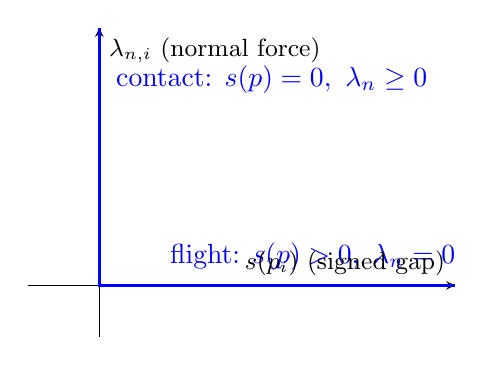
\begin{tikzpicture}
\begin{axis}[axis lines=middle,width=7cm,height=5.5cm,xmin=-1,xmax=5,ymin=-1,ymax=5,
  xlabel={$s(p_i)$ (signed gap)},ylabel={$\lambda_{n,i}$ (normal force)},
  xtick=\empty,ytick=\empty,every axis label/.append style={font=\small}]
  \addplot[very thick,blue] coordinates {(0,5)(0,0)(5,0)};
  \node[blue,right] at (axis cs:0.1,4) {contact: $s(p)=0,\ \lambda_n\ge 0$};
  \node[blue,above] at (axis cs:3,0.1) {flight: $s(p)>0,\ \lambda_n=0$};
\end{axis}
\end{tikzpicture}
\caption{The Signorini condition: the admissible $(s,\lambda_n)$ pairs form an L-shaped set.}
\end{figure}

\begin{intuition}
It is a switch with only two positions. Either the foot is in the air (signed gap $s(p)>0$) and the
force is exactly zero, or the foot is on the ground (signed gap $s(p)=0$) and the force may be any
nonnegative value. The product of the two is always zero; this ``either/or'' is what makes
legged locomotion a \emph{hybrid} problem. Numbers: a foot $2$\,cm above the ground has
$s(p)=+0.02$\,m and can exert $0$\,N; a foot at $s(p)=0$ under a $60$\,kg robot in double support
carries about $294$\,N.
\end{intuition}

% =====================================================================
\section{From Geometric Conditions to Kinematic Constraints \sr}

When a contact is maintained over an interval of time $[t_1, t_2]$, we have $s(p_i(t)) \equiv 0$ (or $d(q(t)) \equiv 0$), which is referred to as \emph{persistent contact}. Over this interval, the geometric unilateral inequality temporarily acts as an equality constraint.

In kinematic analysis, the essential distinction is: \emph{which degrees of freedom of the contact point are restricted?} This leads to \textbf{two fundamental contact models}:
\begin{enumerate}[nosep]
  \item \textbf{Persistent contact with sliding allowed} (sliding or frictionless contact: $1$ scalar constraint along the surface normal);
  \item \textbf{Sticking point contact without slip} (pinned contact: $3$ scalar constraints in all spatial directions).
\end{enumerate}

\subsection{Two contact models in kinematic analysis \sr}

\begin{definition}{Model 1: Persistent contact with sliding allowed}{sliding_model}
The contact point is constrained to stay on the surface, but tangential displacement (sliding) is permitted:
\begin{align}
  \text{position level ($1$ constraint):}\quad & d(q) = n^\top\big(p_c(q) - p_{\text{surf}}\big) = 0, \label{eq:slide_pos}\\
  \text{velocity level ($1$ constraint):}\quad & \dot d(q) = n^\top \dot p_c(q) = n^\top J_c(q)\,v = J_n(q)\,v = 0, \label{eq:slide_vel}\\
  \text{acceleration level ($1$ constraint):}\quad & \ddot d(q) = J_n(q)\,\dot v + \dot J_n(q,v)\,v = 0, \label{eq:slide_acc}
\end{align}
where $J_n(q) = n^\top J_c(q) \in \R^{1 \times n_v}$ is the normal contact Jacobian.
\begin{itemize}[nosep]
  \item \textbf{Tangential velocity:} The tangential velocity $v_t = (I - n n^\top)\dot p_c \in \R^3$ is kinematically \emph{unconstrained} ($v_t \neq 0$ is permitted).
  \item \textbf{Contact force:} The constraint reaction is purely normal, $f_c = \lambda_n n = J_n(q)^\top \lambda_n$ with $\lambda_n \ge 0$ (if frictionless). Under Coulomb sliding friction, a dissipative friction force acts opposite to the tangential slip direction:
  \[
    f_t = -\mu \lambda_n \frac{v_t}{\|v_t\|} \qquad (v_t \neq 0).
  \]
\end{itemize}
\end{definition}

\begin{definition}{Model 2: Sticking point contact without slip}{rigid}
The contact point is completely pinned in 3D space: both normal detachment and tangential sliding are prevented ($v_n = 0$ and $v_t = 0$):
\begin{align}
  \text{position level ($3$ constraints):}\quad & p_c(q) = p_c^0 = \text{const} \in \R^3, \label{eq:stick_pos}\\
  \text{velocity level ($3$ constraints):}\quad & \dot p_c(q) = \Jc(q)\,v = 0, \label{eq:vel}\\
  \text{acceleration level ($3$ constraints):}\quad & \ddot p_c(q) = \Jc(q)\,\dot v+\dot J_c(q,v)\,v = 0, \label{eq:acc}
\end{align}
where $\Jc(q) = \partial p_c/\partial q \in \R^{3 \times n_v}$.
\begin{itemize}[nosep]
  \item \textbf{Tangential velocity:} Tangential motion is completely locked ($v_t = 0$ along with $v_n = 0$).
  \item \textbf{Contact force:} The constraint reaction is a full 3D vector $f_c = \Jc(q)^\top \lambda_c = \lambda_n n + f_t \in \R^3$.
  \item \textbf{Physical validity (admissibility):} The sticking assumption remains physically valid without slip if and only if the force stays inside the static Coulomb friction cone:
  \[
    \lambda_n \ge 0 \qquad \text{and} \qquad \|f_t\| \le \mu\,\lambda_n.
  \]
\end{itemize}
A point contact without slip imposes $3$ scalar constraints; a flat-foot (surface) contact that cannot rotate imposes $6$ (3 position + 3 orientation).
\end{definition}

\begin{table}[ht]
\centering
\small
\renewcommand{\arraystretch}{1.25}
\begin{tabular}{@{}p{3.4cm}p{5.5cm}p{5.5cm}@{}}
\toprule
\textbf{Kinematic feature} & \textbf{Persistent Contact (Sliding Allowed)} & \textbf{Sticking Point Contact (No Slip)} \\
\midrule
Scalar constraints ($m$) & $m = 1$ (normal direction only) & $m = 3$ (all spatial directions) \\
Position condition & $d(q) = n^\top(p_c(q) - p_{\text{surf}}) = 0$ & $p_c(q) = p_c^0 = \text{const}$ \\
Velocity condition & $J_n(q)\,v = 0$ & $\Jc(q)\,v = 0$ \\
Tangential velocity & Free ($v_t = (I - n n^\top)\dot p_c \neq 0$) & Vanishes ($v_t = 0$) \\
Acceleration condition & $J_n\dot v + \dot J_n v = 0$ & $\Jc\dot v + \dot J_c v = 0$ \\
Constraint force & Normal: $f_c = \lambda_n n$ ($+\,f_t$ from sliding) & Full 3D force: $f_c = \lambda_n n + f_t$ \\
Admissibility criterion & $\lambda_n \ge 0$ & $\lambda_n \ge 0$ and $\|f_t\| \le \mu\lambda_n$ \\
Typical application & Ice skating, wheels sliding, low friction & Stance foot in legged walking/running \\
\bottomrule
\end{tabular}
\caption{Kinematic comparison of the two contact models under persistent contact.}
\label{tab:two_contact_models}
\end{table}

\begin{intuition}
Model 1 (sliding) removes only $1$ DoF per contact point, leaving the robot free to glide across the floor. Model 2 (sticking) removes $3$ DoFs, acting as a passive spherical ball-and-socket joint pinned to the ground. In legged locomotion, control designs typically assume Model 2 for all stance feet to ensure reliable propulsion, enforcing the friction cone $\|f_t\|\le\mu\lambda_n$ at every control cycle to prevent transitions into unwanted sliding.
\end{intuition}

\subsection{Single sticking point contact: independence and why $\rank J_c=3$ \sr}

For a single sticking point contact (Model~2), the kinematic constraint at velocity level is:
\begin{equation}\label{eq:single_stick}
  \dot p_c = J_c(q)\,v = 0, \qquad J_c(q) \in \R^{3 \times n_v}.
\end{equation}
Two fundamental questions arise in kinematic contact analysis:
\begin{enumerate}[nosep]
  \item \emph{Are the three scalar constraints independent?}
  \item \emph{Why does the Jacobian $J_c(q)$ always have full row rank, i.e., $\rank J_c(q) = 3$?}
\end{enumerate}

\begin{proposition}{Independence of the three sticking constraints}{stick_indep}
Let $n \in \R^3$ be the surface unit normal, and let $t_1, t_2 \in \R^3$ be two mutually orthogonal unit vectors tangent to the surface, such that $\{n, t_1, t_2\}$ forms a right-handed orthonormal contact frame. The rotation matrix $R = [\,n\;\; t_1\;\; t_2\,]^\top \in SO(3)$ maps global Cartesian coordinates to the contact frame.

Projecting the velocity constraint $\dot p_c = 0$ onto this frame yields:
\begin{equation}\label{eq:stick_decomp}
  R\,\dot p_c = \begin{bmatrix} n^\top \\ t_1^\top \\ t_2^\top \end{bmatrix} J_c(q)\,v = \begin{bmatrix} J_n(q) \\ J_{t_1}(q) \\ J_{t_2}(q) \end{bmatrix} v = \begin{bmatrix} 0 \\ 0 \\ 0 \end{bmatrix}.
\end{equation}
The three scalar equations enforce:
\begin{itemize}[nosep]
  \item $J_n(q)\,v = n^\top \dot p_c = 0$: no motion along the normal (prevents penetration and liftoff, $m=1$);
  \item $J_{t_1}(q)\,v = t_1^\top \dot p_c = 0$: no slip along the first tangent axis ($m=1$);
  \item $J_{t_2}(q)\,v = t_2^\top \dot p_c = 0$: no slip along the second tangent axis ($m=1$).
\end{itemize}
Because $\{n, t_1, t_2\}$ are mutually orthogonal in $\R^3$, $R$ is strictly non-singular ($R^{-1} = R^\top$). Consequently, no row of \eqref{eq:stick_decomp} can ever be written as a linear combination of the other two: the three constraints are \textbf{mutually independent}.
\end{proposition}

\begin{proposition}{Why $\rank J_c(q) = 3$ for a floating-base robot}{rank_jc3}
For a floating-base system, the generalized velocity vector partitions into base linear velocity $\dot p_b \in \R^3$, base angular velocity $\omega_b \in \R^3$, and joint rates $\dot q_j \in \R^n$:
\[
  v = \begin{bmatrix} \dot p_b \\ \omega_b \\ \dot q_j \end{bmatrix} \in \R^{n_v}, \qquad n_v = 6 + n.
\]
The kinematic velocity of any contact point $p_c(q)$ on the robot is given by rigid-body kinematics:
\[
  \dot p_c = \dot p_b + \omega_b \times \big(p_c(q) - p_b\big) + J_{c,j}(q)\,\dot q_j ,
\]
where $J_{c,j}(q) = \partial p_c/\partial q_j \in \R^{3 \times n}$ is the joint Jacobian of the leg. In block-matrix form:
\begin{equation}\label{eq:jc_block}
  J_c(q) = \begin{bmatrix} I_3 & -\big[p_c(q)-p_b\big]_\times & J_{c,j}(q) \end{bmatrix} \in \R^{3 \times (6+n)},
\end{equation}
where $I_3$ is the $3\times 3$ identity matrix and $[a]_\times \in \R^{3\times 3}$ is the skew-symmetric cross-product matrix ($[a]_\times b = a \times b$).
\begin{itemize}[nosep]
  \item The submatrix corresponding to base linear velocity $\dot p_b$ is the $3\times 3$ identity matrix $I_3$.
  \item The rank of a block matrix satisfies $\rank J_c(q) \ge \rank(I_3) = 3$.
  \item Since $J_c(q)$ has only $3$ rows, its row rank cannot exceed $3$. Therefore:
  \begin{equation}
    \rank J_c(q) \equiv 3 \qquad \forall\, q \in \mathcal Q.
  \end{equation}
\end{itemize}
\end{proposition}

\begin{intuition}
Why is a single sticking foot on a floating-base robot immune to kinematic singularities?
Because the floating base has unconstrained translational freedom in $\R^3$: a pure base translation $\dot p_b$ translates the entire robot as a rigid body, moving the foot with identity velocity $\dot p_c = \dot p_b$. Even if the leg joints were completely frozen ($\dot q_j = 0$) or aligned in a singular configuration (e.g.\ fully extended knee), base translation alone spans all $3$ velocity dimensions. Thus, $\rank J_c = 3$ holds identically across the entire configuration space.

\textbf{Fixed base vs.\ floating base:}
For a fixed-base manipulator or leg, $J_c = J_{c,j} \in \R^{3 \times n}$. There, $\rank J_{c,j} = 3$ requires at least $3$ joints and holds only away from internal kinematic singularities ($\det(J_{c,j}J_{c,j}^\top) \neq 0$). On a floating base, the presence of $I_3$ guarantees full row rank unconditionally.
\end{intuition}

\subsection{A fundamental caveat: kinematics is blind to friction \sr}

A critical conceptual pillar in contact mechanics is that \textbf{kinematics is blind to friction}.

\begin{proposition}{Kinematic admissibility vs.\ physical feasibility}{kin_blind}
The kinematic equations for a sticking point contact,
\begin{equation}\label{eq:kin_stick_cond}
  \dot p_c = J_c(q)\,v = 0 \qquad \text{and} \qquad \ddot p_c = J_c(q)\,\dot v + \dot J_c(q,v)\,v = 0,
\end{equation}
are purely geometric relationships between coordinates, velocities, and accelerations.
\begin{itemize}[nosep]
  \item \textbf{Absence of the friction coefficient $\mu$:} The friction coefficient $\mu$ does not appear anywhere in \eqref{eq:kin_stick_cond}. The kinematic condition $J_c(q)v=0$ is strictly identical whether the robot stands on rough asphalt ($\mu \approx 1.0$), polished marble ($\mu \approx 0.2$), or frictionless ice ($\mu = 0$).
  \item \textbf{Implicit assumption of infinite constraint capability:} Kinematics assumes that the constraint is enforced by an ideal bilateral reaction force capable of producing whatever tangential force $f_t \in \R^2$ is required to prevent motion, regardless of any physical bounds.
  \item \textbf{Kinematic vs.\ dynamic validity:} A robot trajectory may be perfectly valid kinematically ($v \in \ker J_c$), yet completely unrealizable physically because the required contact forces cannot be sustained by the ground.
\end{itemize}
\end{proposition}

\begin{intuition}
\textbf{``Kinematics postulates the constraint; dynamics computes the forces required; friction laws decide whether physics allows it.''}

Consider a biped attempting an aggressive acceleration on wet ice versus dry asphalt. Kinematically, the task specification for the stance foot is identical in both environments: the foot must stay planted without slipping ($\dot p_c = 0$).

Kinematics cannot tell you whether the foot will actually hold or slide. To determine physical realizability, one must follow the three-tier hierarchy:
\begin{enumerate}[nosep]
  \item \textbf{Kinematic Level:} Enforce $\Jc v = 0$ and $\Jc \dot v + \dot J_c v = 0$ to identify kinematically admissible accelerations.
  \item \textbf{Dynamic Level:} Solve the equations of motion (the KKT system of Section~\ref{sec:cdyn}) to compute the unique contact force $f_c = \lambda_n n + f_t$ required to prevent the contact point from accelerating.
  \item \textbf{Friction / Contact Mechanics Level:} Check whether the computed force lies inside the Coulomb friction cone (Section~\ref{sec:fric}):
  \[
    \lambda_n \ge 0 \qquad \text{and} \qquad \|f_t\| \le \mu\,\lambda_n.
  \]
\end{enumerate}
If $\|f_t\| > \mu\lambda_n$, nature cannot deliver the tangential force that kinematics presupposed. The sticking assumption breaks down, the constraint $\dot p_c=0$ is violated, and the contact transitions dynamically into sliding (Model~1) or uncontrolled slip. This is precisely why modern Whole-Body Controllers (Section~\ref{sec:wbc}) cannot treat sticking contact as a purely kinematic projection: they must embed the friction cone $\|f_t\| \le \mu\lambda_n$ as an explicit inequality constraint inside a real-time QP optimization.
\end{intuition}

\subsection{Running example: a planar leg \sr}\label{sec:planar_leg}

To consolidate all geometric and kinematic concepts introduced so far, we formulate a running benchmark that illustrates contact geometry, kinematics, and constrained dynamics: a **planar leg**.

\begin{example}{Kinematic and contact analysis of a planar leg}{planar_leg}
\textbf{1. Geometric model and configuration coordinates:}\\
The system consists of a rigid leg of length $l$ attached to an actuated/floating hip located at Cartesian position $(x, z) \in \R^2$ with a point foot at its tip. The leg angle $\theta$ is measured counterclockwise from the downward vertical and is defined positive when the foot moves to the right of the hip ($+x$ direction). The generalized configuration coordinates and velocities are:
\[
  q = \begin{bmatrix} x \\ z \\ \theta \end{bmatrix} \in \R^3 \qquad (n_q = 3), \qquad
  v = \dot q = \begin{bmatrix} \dot x \\ \dot z \\ \dot\theta \end{bmatrix} \in \R^3.
\]

\textbf{2. Point foot forward kinematics:}\\
By trigonometry, the Cartesian position of the point foot in the world frame is:
\begin{equation}\label{eq:leg_foot_pos}
  p_f(q) = \begin{bmatrix} x_f(q) \\ z_f(q) \end{bmatrix} = \begin{bmatrix} x + l\sin\theta \\ z - l\cos\theta \end{bmatrix}.
\end{equation}

\textbf{3. Ground contact and unilateral gap function:}\\
The ground is flat and rigid at $z = 0$, with upward unit normal $n = [0\ \ 1]^\top = e_z$. The unilateral signed gap function $d(q)$ measures the vertical clearance of the point foot from the floor:
\begin{equation}\label{eq:leg_gap}
  d(q) = n^\top\big(p_f(q) - p_{\text{surf}}\big) = z_f(q) - 0 = z - l\cos\theta.
\end{equation}
The physical contact regimes are:
\begin{itemize}[nosep]
  \item $d(q) > 0 \iff z > l\cos\theta$: flight phase (foot in the air, normal force $\lambda_n = 0$);
  \item $d(q) = 0 \iff z = l\cos\theta$: contact active (foot touches the floor, $\lambda_n \ge 0$);
  \item $d(q) < 0 \iff z < l\cos\theta$: interpenetration into the ground (physically forbidden).
\end{itemize}
Under Signorini complementarity:
\begin{equation}
  0 \;\le\; (z - l\cos\theta) \;\perp\; \lambda_n \;\ge\; 0.
\end{equation}

\textbf{4. Contact Jacobians:}\\
Differentiating \eqref{eq:leg_foot_pos} yields the foot velocity $\dot p_f = J_f(q)\,\dot q$, where the foot contact Jacobian is:
\begin{equation}\label{eq:leg_jf}
  J_f(q) = \frac{\partial p_f}{\partial q} = \begin{bmatrix} 1 & 0 & l\cos\theta \\ 0 & 1 & l\sin\theta \end{bmatrix} \in \R^{2 \times 3}.
\end{equation}
The normal contact Jacobian $J_n(q) = \partial d/\partial q = n^\top J_f(q) \in \R^{1 \times 3}$ describes the rate of change of the gap:
\begin{equation}\label{eq:leg_jn}
  \dot d(q) = J_n(q)\,\dot q = \begin{bmatrix} 0 & 1 & l\sin\theta \end{bmatrix} \begin{bmatrix} \dot x \\ \dot z \\ \dot\theta \end{bmatrix} = \dot z + l\sin\theta\,\dot\theta.
\end{equation}

\textbf{5. Two contact models under persistent contact ($d(q) \equiv 0$):}\\
\begin{itemize}[nosep]
  \item \textbf{Model 1 (Persistent contact with sliding allowed):}
  Only normal motion is prevented ($d(q) = z - l\cos\theta = 0$). The velocity constraint is:
  \[
    \dot d = J_n(q)\,v = \dot z + l\sin\theta\,\dot\theta = 0 \implies \dot z = -l\sin\theta\,\dot\theta.
  \]
  The foot slides horizontally along the floor with velocity $\dot x_f = \dot x + l\cos\theta\,\dot\theta \neq 0$. The system retains $3 - 1 = 2$ degrees of freedom $(\dot x, \dot\theta)$.
  \item \textbf{Model 2 (Sticking point foot without slip):}
  Both horizontal and vertical motion are locked ($\dot p_f = 0$):
  \[
    J_f(q)\,v = \begin{bmatrix} 1 & 0 & l\cos\theta \\ 0 & 1 & l\sin\theta \end{bmatrix} \begin{bmatrix} \dot x \\ \dot z \\ \dot\theta \end{bmatrix} = \begin{bmatrix} 0 \\ 0 \end{bmatrix} \implies
    \begin{cases}
      \dot x = -l\cos\theta\,\dot\theta, \\
      \dot z = -l\sin\theta\,\dot\theta.
    \end{cases}
  \]
  Base translation $(\dot x, \dot z)$ is completely slaved to the joint rate $\dot\theta$, leaving $3 - 2 = 1$ degree of freedom ($\nu = \dot\theta$).
\end{itemize}

\textbf{6. Full row rank and independence:}\\
Notice that the foot contact Jacobian decomposes as:
\[
  J_f(q) = \begin{bmatrix} I_2 & J_{f,j}(q) \end{bmatrix} = \begin{bmatrix} 1 & 0 & l\cos\theta \\ 0 & 1 & l\sin\theta \end{bmatrix},
\]
where the leading $2\times 2$ block corresponding to hip linear translation $(\dot x, \dot z)$ is the identity matrix $I_2$.
Therefore, $\rank J_f(q) \equiv 2$ unconditionally across all configurations (Proposition~\ref{prop:rank_jc3}). The normal constraint $J_n$ and tangential constraint $J_t = [1\ \ 0\ \ l\cos\theta]$ are mutually orthogonal and independent (Proposition~\ref{prop:stick_indep}).

\textbf{7. Kinematics is blind to friction:}\\
The kinematic equations $\dot x = -l\cos\theta\,\dot\theta$ and $\dot z = -l\sin\theta\,\dot\theta$ have zero dependence on the friction coefficient $\mu$. Whether the foot actually sticks without slipping depends dynamically on whether the contact force satisfies $|f_x| \le \mu f_z$ with $f_z \ge 0$.

\begin{center}
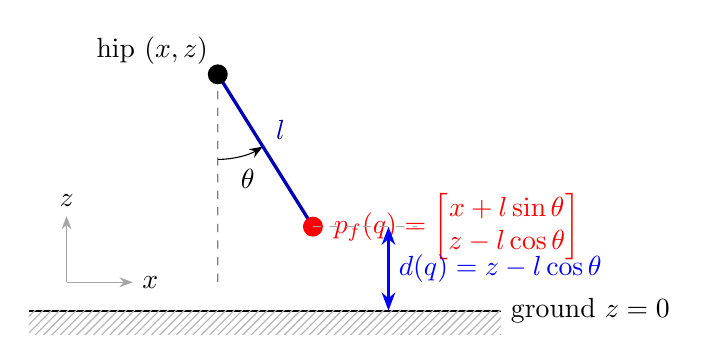
\begin{tikzpicture}[>=Stealth,scale=1.2]
  % Ground
  \draw[thick] (-0.8,0) -- (4.2,0);
  \fill[pattern=north east lines,pattern color=gray!60] (-0.8,-0.25) rectangle (4.2,0);
  \node[right,black] at (4.2,0) {ground $z=0$};

  \def\hx{1.2}
  \def\hz{2.5}
  \def\len{1.9}
  \def\ang{32}

  \coordinate (H) at (\hx,\hz);
  \coordinate (F) at ({\hx + \len*sin(\ang)},{\hz - \len*cos(\ang)});

  % Reference vertical dashed line
  \draw[dashed,gray] (H) -- (\hx,0.3);
  \draw[->] (\hx,{\hz-0.9}) arc (-90:{-90+\ang}:0.9);
  \node at ({\hx + 1.15*sin(\ang/2)},{\hz - 1.15*cos(\ang/2)}) {$\theta$};

  % Leg link
  \draw[very thick,blue!70!black] (H) -- (F) node[midway,above right] {$l$};

  % Hip mass/base
  \fill[black] (H) circle (3pt) node[above left] {hip $(x,z)$};

  % Foot point
  \fill[red] (F) circle (3pt) node[right=4pt] {$p_f(q) = \begin{bmatrix} x + l\sin\theta \\ z - l\cos\theta \end{bmatrix}$};

  % Height / gap dimension
  \draw[dashed,gray!70] (F) -- ({\hx + \len*sin(\ang) + 1.1},{\hz - \len*cos(\ang)});
  \draw[<->,thick,blue] ({\hx + \len*sin(\ang) + 0.8},0) -- ({\hx + \len*sin(\ang) + 0.8},{\hz - \len*cos(\ang)})
    node[midway,right] {$d(q) = z - l\cos\theta$};

  % Coordinates indicator
  \draw[->,thin,gray!70] (-0.4,0.3) -- (0.3,0.3) node[right,black] {$x$};
  \draw[->,thin,gray!70] (-0.4,0.3) -- (-0.4,1.0) node[above,black] {$z$};
\end{tikzpicture}
\end{center}
\end{example}

\subsection{Multiple contacts, constraint rank, and static indeterminacy \sr}

\begin{intuition}
The constraint is imposed at \emph{acceleration} level because that is the level at which
the equations of motion \eqref{eq:eom} live. If the foot velocity is zero now and its
acceleration is zero, it stays at zero. Counting for a quadruped with four point feet:
$4\times 3=12$ constraints on $n_v=18$ velocities leaves $18-12=6$ free generalized
velocities. For a biped with two flat feet, $2\times 6=12$ constraints on $n_v=18$: again $6$.
\end{intuition}

\begin{proposition}{Constraint rank}{rank}
If $\Jc\in\R^{m\times n_v}$ has full row rank $m$ (the contacts are independent), the
constraint \eqref{eq:vel} defines a smooth $(n_v-m)$-dimensional manifold of admissible
velocities, $\ker\Jc$. If $\Jc$ loses rank (e.g.\ redundant contacts, or a fully stretched
leg) then $\Jc M^{-1}\Jc^\top$ is singular and the contact forces are not uniquely determined.
\end{proposition}

\begin{intuition}
Imagine a table with four legs on perfectly flat ground: any three legs would already hold it
and the fourth only adds redundancy. The load can then be shared among legs in infinitely
many ways, so statics alone cannot say how much each leg carries. This is the same rank
drop as above, and it is why practical controllers choose the distribution by optimization.
\end{intuition}

Numerical drift in integrating \eqref{eq:acc} is usually handled by replacing it with the
stabilized version (see Appendix~\ref{app:baumgarte}).

% =====================================================================
\section{Constrained Dynamics \sr}\label{sec:cdyn}

To compute the motion of a mechanical system subject to constraints, one must combine the equations of motion with the constraints differentiated up to acceleration level. This yields a structured linear algebraic system in the unknowns (generalized accelerations and constraint reaction forces), known in analytical mechanics and multibody dynamics as the \textbf{augmented form} (or \emph{augmented system} / \emph{saddle-point / KKT form}).

\subsection{The augmented form in generalized coordinates $(\ddot q, \lambda)$ \sr}

Consider a mechanical system described by generalized coordinates $q \in \R^{n_q}$, with unconstrained equations of motion:
\begin{equation}\label{eq:eom_unconstrained}
  M(q)\,\ddot q + h(q,\dot q) = \tau + F_{\mathrm{con}},
\end{equation}
where $M(q) \succ 0$ is the symmetric positive-definite inertia matrix, $h(q,\dot q) = c(q,\dot q) + g(q)$ collects Coriolis, centrifugal, and gravitational forces, and $\tau \in \R^{n_q}$ represents the generalized actuation torques.

Suppose the system is constrained by $m$ independent holonomic constraints $\varphi(q) = 0$, with constraint Jacobian $J(q) = \partial\varphi/\partial q \in \R^{m \times n_q}$.
\begin{itemize}[nosep]
  \item By d'Alembert's principle (Proposition~\ref{prop:work}), the constraint forces do zero virtual work on any admissible velocity:
  \begin{equation}
    F_{\mathrm{con}} = J(q)^\top \lambda,
  \end{equation}
  where $\lambda \in \R^m$ is the vector of \textbf{Lagrange multipliers} representing the magnitude of the constraint forces.
  \item Differentiating the constraint $\varphi(q) = 0$ twice with respect to time enforces the constraint at acceleration level (Proposition~\ref{prop:accadm}):
  \begin{align}
    \dot\varphi(q) &= J(q)\,\dot q = 0, \label{eq:velo_holo}\\
    \ddot\varphi(q) &= J(q)\,\ddot q + \dot J(q,\dot q)\,\dot q = 0. \label{eq:acc_holo}
  \end{align}
\end{itemize}

\begin{theorem}{Augmented form of the constrained dynamics}{augmented_form}
Stacking the unconstrained equations of motion \eqref{eq:eom_unconstrained} and the acceleration-level constraint \eqref{eq:acc_holo} yields a linear $(n_q + m) \times (n_q + m)$ system in the unknowns $(\ddot q, \lambda)$:
\begin{equation}\label{eq:augmented_sys}
\begin{bmatrix}
  M(q) & -J(q)^\top \\
  J(q) & 0
\end{bmatrix}
\begin{bmatrix}
  \ddot q \\
  \lambda
\end{bmatrix}
=
\begin{bmatrix}
  \tau - h(q,\dot q) \\
  -\dot J(q,\dot q)\,\dot q
\end{bmatrix}.
\end{equation}
Equation \eqref{eq:augmented_sys} is the \textbf{augmented form} of the constrained equations of motion.

If $J(q)$ has full row rank $m$, the augmented matrix is non-singular, and the closed-form solution is:
\begin{align}
  \Lambda(q) &= \big(J(q) M(q)^{-1} J(q)^\top\big)^{-1}, \label{eq:lambda_gen}\\
  \lambda &= -\Lambda(q)\Big(J(q) M(q)^{-1}\big(\tau - h(q,\dot q)\big) + \dot J(q,\dot q)\,\dot q\Big), \label{eq:lambda_sol}\\
  \ddot q &= M(q)^{-1}\big(\tau - h(q,\dot q) + J(q)^\top \lambda\big). \label{eq:qddot_sol}
\end{align}
\end{theorem}
\begin{proof}
Since $M(q) \succ 0$, $M(q)$ is invertible. From the first row of \eqref{eq:augmented_sys}:
\[
  \ddot q = M(q)^{-1}\big(\tau - h(q,\dot q) + J(q)^\top \lambda\big).
\]
Substituting this expression into the second block row $J(q)\ddot q = -\dot J(q,\dot q)\dot q$:
\[
  J(q) M(q)^{-1}\big(\tau - h(q,\dot q)\big) + J(q) M(q)^{-1} J(q)^\top \lambda = -\dot J(q,\dot q)\,\dot q.
\]
Because $M \succ 0$ and $J$ has full row rank $m$, the Delassus matrix $J(q) M(q)^{-1} J(q)^\top \in \R^{m \times m}$ is symmetric positive-definite, and hence invertible. Its inverse is the operational-space inertia $\Lambda(q)$. Solving for $\lambda$ yields \eqref{eq:lambda_sol}, and substituting $\lambda$ back into the first equation gives \eqref{eq:qddot_sol}.
\end{proof}

\begin{intuition}
\textbf{Why is it called the augmented form?}
Instead of eliminating the constraints to identify a minimal set of $(n_q - m)$ coordinates (which can be geometrically complicated or impossible globally), we \emph{augment} the system unknowns by appending the $m$ Lagrange multipliers $\lambda$ to the accelerations $\ddot q$. This transforms non-linear constrained dynamics into a structured linear system that can be solved at each time step.
\end{intuition}

\subsection{Floating-base contact dynamics in $(\dot v, f_c)$ \sr}

For a legged robot with a floating base, the configuration manifold is $SE(3) \times \R^n$. The generalized velocities are $v = (v_b, \dot q_j) \in \R^{n_v}$ with base twist $v_b \in \R^6$, the acceleration is $\dot v$, and the contact force/wrench vector $f_c \in \R^m$ plays the role of the Lagrange multipliers $\lambda$ (with contact generalized force $F_{\mathrm{con}} = \Jc(q)^\top f_c$).

Stacking the floating-base equations of motion \eqref{eq:eom} and the contact acceleration constraint \eqref{eq:acc}:
\begin{equation}\label{eq:kkt}
\begin{bmatrix} M & -\Jc^{\top}\\ \Jc & 0\end{bmatrix}
\begin{bmatrix}\dot v\\ f_c\end{bmatrix}
=
\begin{bmatrix} S^{\top}\tau-h\\ -\dot J_c v\end{bmatrix}.
\end{equation}
This is the floating-base formulation of the augmented form \eqref{eq:augmented_sys}. When $\Jc$ has full row rank, its solution is identical in structure:
\begin{align}
  \Lambda &= \big(\Jc M^{-1}\Jc^\top\big)^{-1}, \label{eq:lambda}\\
  f_c &= -\Lambda\Big(\Jc M^{-1}(S^\top\tau-h)+\dot J_c v\Big), \label{eq:fc}\\
  \dot v &= M^{-1}\big(S^\top\tau-h+\Jc^\top f_c\big). \label{eq:vdot}
\end{align}

\begin{intuition}
The matrix $\Lambda$ is the \emph{operational-space inertia} seen at the contact points:
how much ``mass'' the robot opposes to an acceleration of the feet. Equation \eqref{eq:fc}
reads: the contact force is whatever is needed to cancel the acceleration the feet would
otherwise get from torques and gravity ($\Jc M^{-1}(S^\top\tau-h)$) and from the motion
itself ($\dot J_c v$). Note that $f_c$ is \emph{not} chosen by the robot: given $q,v,\tau$
it is determined.
\end{intuition}

\begin{definition}{Dynamically consistent inverse and null-space projector}{dci}
\begin{equation}
  \Jb=M^{-1}\Jc^\top\Lambda,\qquad N=I-\Jb\,\Jc .
\end{equation}
$\Jb$ is the $M^{-1}$-weighted pseudoinverse of $\Jc$ and $N$ the corresponding projector.
\end{definition}

\begin{proposition}{Constrained dynamics via projection}{proj}
With the definitions above,
\begin{align}
  \dot v &= N\,M^{-1}(S^\top\tau-h)-\Jb\,\dot J_c v, \label{eq:vdotN}\\
  N^{\top}\big(M\dot v+h-S^\top\tau\big)&=0 , \label{eq:nulldyn}
\end{align}
and $N^\top\Jc^\top=0$: the projected equation \eqref{eq:nulldyn} does not contain the
contact forces.
\end{proposition}
\begin{proof}
Substituting \eqref{eq:fc} in \eqref{eq:vdot} yields $M^{-1}(S^\top\tau-h)-\Jb\big(\Jc M^{-1}(S^\top\tau-h)+\dot J_c v\big)$,
which is \eqref{eq:vdotN}. For the last claim, $\Jb^\top=\Lambda\Jc M^{-1}$ so
$\Jc^\top\Jb^\top\Jc^\top=\Jc^\top\Lambda\Jc M^{-1}\Jc^\top=\Jc^\top$ and therefore
$N^\top\Jc^\top=\Jc^\top-\Jc^\top\Jb^\top\Jc^\top=0$. Multiplying \eqref{eq:eom} by $N^\top$
removes $\Jc^\top f_c$.
\end{proof}

\begin{intuition}
Two ways to look at the same constrained system. Equation \eqref{eq:vdotN}: take the
unconstrained acceleration and remove its component that would move the feet. Equation
\eqref{eq:nulldyn}: look only at the directions in which the contact forces cannot act;
there, forces vanish from the picture and what remains is the pure ``internal'' motion.
The weighting by $M^{-1}$ makes the projection \emph{dynamically consistent}: the
projected motion does not generate accelerations at the contacts.
\end{intuition}

\subsection{Running example: planar leg constrained dynamics \sr}\label{sec:planar_leg_dyn}

We now apply the augmented form and floating-base constrained dynamics to the running example introduced in Section~\ref{sec:planar_leg}.

\begin{example}{Constrained dynamics of a planar leg with hip mass $m_h$}{planar_leg_dyn}
\textbf{1. Mass model and unconstrained equations of motion:}\\
We model the system with a lumped point mass $m_h$ located at the floating hip $(x, z)$. The rigid leg of length $l$ has pitch angle $\theta$ and is modeled as a massless link (with optional leg pitch inertia $I \ge 0$ about the hip). The generalized coordinates are:
\[
  q = \begin{bmatrix} x \\ z \\ \theta \end{bmatrix} \in \R^3, \qquad
  v = \dot q = \begin{bmatrix} \dot x \\ \dot z \\ \dot\theta \end{bmatrix} \in \R^3.
\]
The kinetic energy is:
\begin{equation}
  T(q,\dot q) = \frac{1}{2}m_h\big(\dot x^2 + \dot z^2\big) + \frac{1}{2}I\,\dot\theta^2,
\end{equation}
and the gravitational potential energy is $V(q) = m_h g z$ (with gravity $g = 9.81\,\text{m/s}^2$ acting downward along $-e_z$). The generalized mass matrix is diagonal and state-independent:
\begin{equation}
  M(q) = \begin{bmatrix} m_h & 0 & 0 \\ 0 & m_h & 0 \\ 0 & 0 & I \end{bmatrix},
\end{equation}
and the nonlinear Coriolis and gravitational forces reduce to:
\begin{equation}
  c(q,\dot q) = 0, \qquad g(q) = \frac{\partial V}{\partial q} = \begin{bmatrix} 0 \\ m_h g \\ 0 \end{bmatrix} \implies h(q,\dot q) = \begin{bmatrix} 0 \\ m_h g \\ 0 \end{bmatrix}.
\end{equation}
The base translation $(x,z)$ is unactuated, while the hip joint provides an actuation torque $\tau_\theta$:
\begin{equation}
  \tau_{\text{gen}} = S^\top \tau_\theta = \begin{bmatrix} 0 \\ 0 \\ \tau_\theta \end{bmatrix}, \qquad S = \begin{bmatrix} 0 & 0 & 1 \end{bmatrix}.
\end{equation}

\textbf{2. Sticking contact constraint at the foot:}\\
Under the sticking foot condition (Model~2 in Section~\ref{sec:planar_leg}), the foot position $p_f(q) = [x + l\sin\theta,\ z - l\cos\theta]^\top$ is stationary: $\dot p_f = J_f(q)\dot q = 0$, with:
\begin{equation}
  J_f(q) = \begin{bmatrix} 1 & 0 & l\cos\theta \\ 0 & 1 & l\sin\theta \end{bmatrix}.
\end{equation}
Differentiating with respect to time enforces the constraint at acceleration level:
\begin{equation}\label{eq:leg_acc_con}
  \ddot p_f = J_f(q)\,\ddot q + \dot J_f(q,\dot q)\,\dot q = 0, \qquad
  \dot J_f(q,\dot q)\,\dot q = \begin{bmatrix} -l\sin\theta\,\dot\theta^2 \\ l\cos\theta\,\dot\theta^2 \end{bmatrix}.
\end{equation}
The constraint reaction forces at the foot are represented by the Lagrange multipliers $\lambda = [\lambda_x,\ \lambda_z]^\top$ (i.e., the contact force vector $f_c = [f_x,\ f_z]^\top$), which exert generalized forces:
\begin{equation}
  F_{\mathrm{con}} = J_f(q)^\top \lambda = \begin{bmatrix} 1 & 0 \\ 0 & 1 \\ l\cos\theta & l\sin\theta \end{bmatrix} \begin{bmatrix} \lambda_x \\ \lambda_z \end{bmatrix} = \begin{bmatrix} \lambda_x \\ \lambda_z \\ l(\lambda_x\cos\theta + \lambda_z\sin\theta) \end{bmatrix}.
\end{equation}

\textbf{3. The augmented form:}\\
Stacking the unconstrained dynamics \eqref{eq:eom_unconstrained} and the acceleration constraint \eqref{eq:leg_acc_con} yields the augmented $(3+2) \times (3+2)$ linear system:
\begin{equation}\label{eq:leg_augmented_kkt}
\begin{bmatrix}
  m_h & 0 & 0 & -1 & 0 \\
  0 & m_h & 0 & 0 & -1 \\
  0 & 0 & I & -l\cos\theta & -l\sin\theta \\
  1 & 0 & l\cos\theta & 0 & 0 \\
  0 & 1 & l\sin\theta & 0 & 0
\end{bmatrix}
\begin{bmatrix}
  \ddot x \\ \ddot z \\ \ddot\theta \\ \lambda_x \\ \lambda_z
\end{bmatrix}
=
\begin{bmatrix}
  0 \\ -m_h g \\ \tau_\theta \\ l\sin\theta\,\dot\theta^2 \\ -l\cos\theta\,\dot\theta^2
\end{bmatrix}.
\end{equation}
The determinant of the augmented saddle-point matrix is:
\begin{equation}
  \det \begin{bmatrix} M & -J_f^\top \\ J_f & 0 \end{bmatrix} = m_h\big(I + m_h l^2\big).
\end{equation}
For any $m_h > 0$ and $l > 0$, the system is strictly non-singular even in the purely massless leg case ($I = 0$).

\textbf{4. Closed-form solution for point mass $m_h$ at the hip ($I = 0$):}\\
Solving \eqref{eq:leg_augmented_kkt} analytically for the ideal point-mass hip model ($I = 0$) gives:
\begin{itemize}[nosep]
  \item \textbf{Inverted pendulum angular acceleration:}
  \begin{equation}\label{eq:leg_thetaddot}
    \ddot\theta = \frac{g}{l}\sin\theta + \frac{\tau_\theta}{m_h l^2}.
  \end{equation}
  The sticking foot constraint transforms the floating leg into a classical inverted pendulum pivoting about the contact point $(x_f, z_f)$.
  \item \textbf{Hip Cartesian accelerations:}
  \begin{align}
    \ddot x &= l\sin\theta\,\dot\theta^2 - l\cos\theta\,\ddot\theta = l\sin\theta\,\dot\theta^2 - \frac{g}{2}\sin(2\theta) - \frac{\tau_\theta}{m_h l}\cos\theta, \label{eq:leg_xddot}\\
    \ddot z &= -l\cos\theta\,\dot\theta^2 - l\sin\theta\,\ddot\theta = -l\cos\theta\,\dot\theta^2 - g\sin^2\theta - \frac{\tau_\theta}{m_h l}\sin\theta. \label{eq:leg_zddot}
  \end{align}
  \item \textbf{Contact reaction forces (Lagrange multipliers):}
  From Newton's second law for the hip point mass ($m_h \ddot x = \lambda_x$ and $m_h (\ddot z + g) = \lambda_z$):
  \begin{align}
    \lambda_x &= m_h \ddot x = m_h l\sin\theta\,\dot\theta^2 - \frac{1}{2}m_h g\sin(2\theta) - \frac{\tau_\theta}{l}\cos\theta, \label{eq:leg_lambdax}\\
    \lambda_z &= m_h(\ddot z + g) = -m_h l\cos\theta\,\dot\theta^2 + m_h g\cos^2\theta - \frac{\tau_\theta}{l}\sin\theta. \label{eq:leg_lambdaz}
  \end{align}
\end{itemize}

\textbf{5. Physical interpretation and contact validity:}\\
\begin{itemize}[nosep]
  \item \textbf{Torque transmission:} Row~3 of \eqref{eq:leg_augmented_kkt} gives $\tau_\theta = -l(\lambda_x\cos\theta + \lambda_z\sin\theta)$. Since the leg has zero inertia, any actuator torque $\tau_\theta$ produces an immediate reaction force moment at the foot.
  \item \textbf{Unilateral condition (no liftoff):} The foot remains on the ground if and only if $\lambda_z \ge 0$, which requires:
  \begin{equation}
    m_h g\cos^2\theta \;\ge\; m_h l\cos\theta\,\dot\theta^2 + \frac{\tau_\theta}{l}\sin\theta.
  \end{equation}
  If the centrifugal pull ($m_h l\cos\theta\,\dot\theta^2$) or hip torque pulling upward exceeds the downward gravity contribution $m_h g\cos^2\theta$, $\lambda_z$ becomes negative and the foot takes off.
  \item \textbf{Coulomb friction cone (no slip):} Sticking contact requires $|\lambda_x| \le \mu \lambda_z$. If $|\lambda_x| > \mu \lambda_z$, the foot slips, invalidating the kinematic assumption $\dot p_f = 0$.
\end{itemize}

\begin{center}
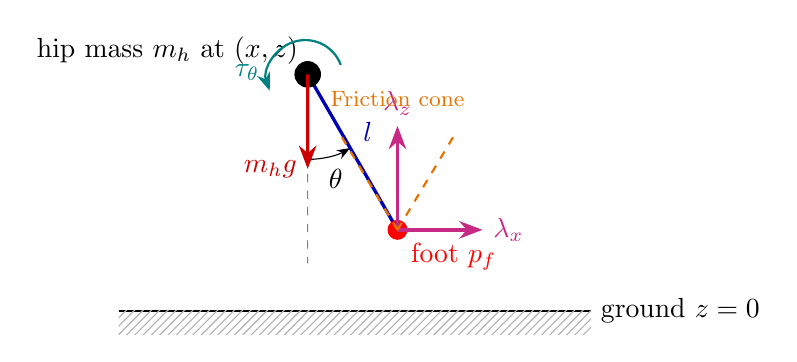
\begin{tikzpicture}[>=Stealth,scale=1.2]
  % Ground
  \draw[thick] (-0.8,0) -- (4.2,0);
  \fill[pattern=north east lines,pattern color=gray!60] (-0.8,-0.25) rectangle (4.2,0);
  \node[right,black] at (4.2,0) {ground $z=0$};

  \def\hx{1.2}
  \def\hz{2.5}
  \def\len{1.9}
  \def\ang{30}

  \coordinate (H) at (\hx,\hz);
  \coordinate (F) at ({\hx + \len*sin(\ang)},{\hz - \len*cos(\ang)});

  % Reference vertical dashed line
  \draw[dashed,gray] (H) -- (\hx,0.5);
  \draw[->] (\hx,{\hz-0.9}) arc (-90:{-90+\ang}:0.9);
  \node at ({\hx + 1.15*sin(\ang/2)},{\hz - 1.15*cos(\ang/2)}) {$\theta$};

  % Leg link
  \draw[very thick,blue!70!black] (H) -- (F) node[midway,above right] {$l$};

  % Hip mass mh
  \fill[black] (H) circle (4pt) node[above left] {hip mass $m_h$ at $(x,z)$};

  % Gravity force at hip
  \draw[->,very thick,red!80!black] (H) -- (\hx,{\hz-1.0}) node[left] {$m_h g$};

  % Hip actuation torque
  \draw[->,thick,teal] ({\hx+0.35},{\hz+0.1}) arc (20:200:0.4) node[above left] {$\tau_\theta$};

  % Foot point
  \fill[red] (F) circle (3pt) node[below right=2pt] {foot $p_f$};

  % Contact forces lambda_x, lambda_z
  \draw[->,very thick,magenta!80!black] (F) -- ($(F) + (0.9,0)$) node[right] {$\lambda_x$};
  \draw[->,very thick,magenta!80!black] (F) -- ($(F) + (0,1.1)$) node[above] {$\lambda_z$};

  % Friction cone at foot
  \draw[dashed,orange!90!black,thick] (F) -- ($(F) + (-0.6,1.0)$);
  \draw[dashed,orange!90!black,thick] (F) -- ($(F) + (0.6,1.0)$);
  \node[orange!90!black,above] at ($(F) + (0,1.2)$) {\footnotesize Friction cone};
\end{tikzpicture}
\end{center}
\end{example}

% % =====================================================================
% \section{Underactuation and the Role of Contact Forces \sr}

% Split the equations of motion into base rows (index $b$, first six) and joint rows ($j$):
% \begin{align}
%   M_b\dot v + h_b &= {\Jc}^{\top}_{b} f_c \label{eq:base}\\
%   M_j\dot v + h_j &= \tau + {\Jc}^{\top}_{j} f_c . \label{eq:joint}
% \end{align}
% The base rows contain \emph{no torque}.

% \begin{proposition}{Centroidal (Newton--Euler) dynamics}{cent}
% Let $m$ be the total mass, $c$ the centre of mass, $g=(0,0,-9.81)$ m/s$^2$, $l$ and $k_G$
% the linear and angular momentum about $c$. Then
% \begin{equation}\label{eq:centroidal}
%   \dot l = m g+\sum_{i=1}^k f_i,\qquad
%   \dot k_G=\sum_{i=1}^k (p_i-c)\times f_i .
% \end{equation}
% \end{proposition}

% \begin{intuition}
% These are Newton and Euler for the whole robot: the total force is gravity plus the sum of
% ground reactions, and the total torque about the centre of mass is the sum of the moments of
% those reactions. No matter how the legs move internally, the \emph{only} way to change the
% body's overall momentum is through $f_i$. Number: for a $60$\,kg robot standing still, the
% vertical contact forces must add up to $mg\approx 588.6$\,N.
% \end{intuition}

% \begin{proposition}{How many contacts are needed?}{cnt}
% Write \eqref{eq:centroidal} as $\dot{\mathcal H}-\mathcal H_g=G\,f_c$ with the \emph{grasp
% matrix} $G\in\R^{6\times 3k}$. For point contacts, $\rank G=6$ requires at least $k=3$
% non-collinear contacts. With $k=2$ point contacts, the moment about the line through the two
% points cannot be produced.
% \end{proposition}

% \begin{intuition}
% A point-foot biped cannot stand still on the spot: it would need to generate a torque about
% the axis through its two feet and has no way to do so, like trying to balance a broom on
% two fingertips side by side. Flat feet fix this by providing a \emph{wrench}
% (force+torque) instead of a single force: that is the topic of the next section.
% \end{intuition}

% % =====================================================================
% \section{Contact Forces: Friction Cones and Contact Wrenches \sr}\label{sec:fric}

% \subsection{Coulomb friction for point contacts \sr}

% \begin{definition}{Coulomb friction cone}{cone}
% For a point contact with normal $n$, tangent plane spanned by $t_1,t_2$ and friction
% coefficient $\mu\ge0$, the admissible forces are
% \begin{equation}\label{eq:cone}
%   \mathcal{K}_\mu=\Big\{f=f_n n+f_t\;:\; f_n\ge0,\;\; \|f_t\|_2\le\mu f_n\Big\}.
% \end{equation}
% It is a second-order (convex) cone.
% \end{definition}

% \begin{figure}[ht]
% \centering
% \begin{tikzpicture}[>=Stealth,scale=1.1]
%   \draw[->] (-3,0) -- (3,0) node[right] {$f_t$};
%   \draw[->] (0,0) -- (0,3.3) node[above] {$f_n$};
%   \fill[blue!12] (0,0) -- (-1.8,3) -- (1.8,3) -- cycle;
%   \draw[very thick,blue] (-1.8,3) -- (0,0) -- (1.8,3);
%   \draw[->,red,very thick] (0,0) -- (0.7,2.2) node[right] {$f$ (sticks)};
%   \draw[->,orange!80!black,very thick] (0,0) -- (2.4,2.0) node[right] {$f'$ (slips)};
%   \draw (0,1) arc (90:59:1);
%   \node at (0.35,1.35) {\small $\arctan\mu$};
%   \node[blue] at (-1.9,1.2) {$\|f_t\|=\mu f_n$};
% \end{tikzpicture}
% \caption{Section of the friction cone in the $(f_t,f_n)$ plane ($\mu=0.6$). Forces inside the cone are sustainable without slipping; outside it the foot slides.}
% \end{figure}

% \begin{intuition}
% The cone encodes everyday experience: the harder you press (large $f_n$), the more sideways
% push the contact withstands, in proportion to $\mu$. Numbers: $60$\,kg robot in double
% support, $f_n\approx 294.3$\,N per foot, $\mu=0.5$: each foot can resist a tangential force
% up to $\mu f_n\approx 147$\,N before slipping. If the planned $f_t$ were $200$\,N, the
% foot would slide.
% \end{intuition}

% \begin{definition}{Linearized friction cone (pyramid)}{pyr}
% To obtain linear constraints, replace $\mathcal K_\mu$ with the cone generated by
% $n_g$ edge vectors,
% $f=\sum_{j=1}^{n_g}\beta_j w_j,\ \beta_j\ge0$, with $w_j=n+\mu'(\cos\theta_j t_1+\sin\theta_j t_2)$.
% With $4$ edges and $\mu'=\mu$ the pyramid is \emph{inscribed} in the cone (more conservative);
% the \emph{box} $|f_{t_1}|\le\mu f_n,\ |f_{t_2}|\le\mu f_n$ \emph{circumscribes} it
% (less conservative, may allow slipping), and $|f_{t_1}|,|f_{t_2}|\le \tfrac{\mu}{\sqrt2}f_n$ is the box inscribed in the cone.
% \end{definition}

% \subsection{Surface contacts: the contact wrench cone \sr}

% For a flat foot with sole $[-\ell_x,\ell_x]\times[-\ell_y,\ell_y]$ in the foot frame,
% contact is described by a wrench $(f,\tau)\in\R^6$ at the sole origin.

% \begin{theorem}{Contact wrench cone of a rectangular foot}{cwc}
% Let $\Pi$ be the foot sole, $f_z\ge0$ the normal force and $(f_x,f_y)$ the tangential force.
% A wrench $(f,\tau)$ is realizable by unilateral, Coulomb-limited forces distributed on $\Pi$
% iff
% \begin{align}
%   & f_z\ge0,\qquad \sqrt{f_x^2+f_y^2}\le\mu f_z, \label{eq:cwc1}\\
%   & |\tau_x|\le \ell_y f_z,\qquad |\tau_y|\le \ell_x f_z, \label{eq:cwc2}\\
%   & |\tau_z|\le \mu(\ell_x+\ell_y)f_z \ \ \text{(up to the standard additional coupling terms)}.\label{eq:cwc3}
% \end{align}
% The centre of pressure is $x_{\mathrm{cop}}=-\tau_y/f_z,\ y_{\mathrm{cop}}=\tau_x/f_z$, and
% \eqref{eq:cwc2} says exactly that it lies inside $\Pi$.
% \end{theorem}
% \begin{proof}[Sketch for \eqref{eq:cwc2}]
% With forces $f_i$ at points $(x_i,y_i,0)$ of the sole, $\tau_x=\sum_i y_i f_{z,i}$ and
% $\tau_y=-\sum_i x_i f_{z,i}$. With $f_{z,i}\ge0$ and $|x_i|\le\ell_x$, $|y_i|\le\ell_y$ we get
% $|\tau_y|\le\ell_x\sum_i f_{z,i}=\ell_x f_z$ and similarly for $\tau_x$. Conversely any
% $(\tau_x,\tau_y)$ satisfying the bounds is produced by a suitable distribution of $f_{z,i}$.
% \end{proof}

% \begin{figure}[ht]
% \centering
% \begin{tikzpicture}[>=Stealth,scale=1.2]
%   \draw[thick,fill=gray!15] (-1.6,-0.8) rectangle (1.6,0.8);
%   \draw[->] (-2.2,0) -- (2.4,0) node[right] {$x$};
%   \draw[->] (0,-1.3) -- (0,1.4) node[above] {$y$};
%   \fill[red] (0.6,0.3) circle (2.5pt) node[above right] {CoP};
%   \node at (1.6,-1.05) {$\ell_x$};
%   \node at (-1.95,0.8) {$\ell_y$};
%   \node[gray!50!black] at (0,-0.55) {\small foot sole $\Pi$};
% \end{tikzpicture}
% \caption{The centre of pressure must stay inside the sole $\Pi$ (here $\ell_x=1.6,\ \ell_y=0.8$ in drawing units).}
% \end{figure}

% \begin{intuition}
% A flat foot can ``push at a point that is not under the ankle''. As long as that point (the
% centre of pressure) remains under the sole, the foot does not tip over its edge. Numbers:
% $f_z=294.3$\,N, $\ell_x=10$\,cm: $|\tau_y|\le 0.10\cdot294.3\approx 29.4$\,Nm. Above this
% torque the foot starts to roll about its toe or heel, which is the same
% physics as the Zero Moment Point condition used in classical biped walking.
% \end{intuition}

% \photoph{Photo of a humanoid foot / sole with force--torque sensor, or of a robot stepping}{?}

% % =====================================================================
% \section{Inverse Dynamics under Contact Constraints \sr}\label{sec:wbc}

% The goal is to compute torques that realize a desired task acceleration while keeping the
% contacts fixed and the contact forces admissible.

% \begin{theorem}{Torques for a desired constrained acceleration}{id}
% Let $\dot v^*$ satisfy $\Jc\dot v^*+\dot J_c v=0$. The torques $\tau$ reproducing it exist
% iff
% \begin{equation}\label{eq:feas}
%   N^\top(M\dot v^*+h)\in\operatorname{range}\big(N^\top S^\top\big),
% \end{equation}
% and in that case $\tau=(N^\top S^\top)^{+}N^\top(M\dot v^*+h)$ (plus null-space terms),
% with contact forces
% \begin{equation}
%   f_c=\Jb^{\top}\big(M\dot v^*+h-S^\top\tau\big).
% \end{equation}
% \end{theorem}
% \begin{proof}
% Projecting \eqref{eq:eom} with $N^\top$ cancels $\Jc^\top f_c$ (Proposition~\ref{prop:proj}),
% leaving the linear system $N^\top S^\top\tau=N^\top(M\dot v^*+h)$ in $\tau$, solvable iff
% \eqref{eq:feas} holds. Having $\tau$, from \eqref{eq:eom}
% $\Jc^\top f_c=M\dot v^*+h-S^\top\tau$; multiplying by $\Jb^\top$ and using
% $\Jb^\top\Jc^\top=\Lambda\Jc M^{-1}\Jc^\top=I$ gives $f_c$.
% \end{proof}

% \begin{intuition}
% The torques have to do two jobs at once: produce the desired motion and make the
% ground reactions come out right. Condition \eqref{eq:feas} says that the desired motion
% is possible only if it does not require a force the robot has no actuator for, for
% instance a base acceleration that would demand pulling the feet \emph{off} the ground
% (see the unilateral constraint below).
% \end{intuition}

% Because friction cones, unilaterality and torque limits are inequalities, the practical
% formulation is a quadratic program solved at every control cycle.

% \begin{algorithm}{Whole-body inverse dynamics as a QP}{wbc}
% At each control step, given $(q,v)$ and a desired task acceleration $a^*$ for a task
% Jacobian $J_t$:
% \begin{align*}
%   \min_{\dot v,\ \tau,\ f_c}\quad & \big\|J_t\dot v+\dot J_t v-a^*\big\|^2_W+\varepsilon\big(\|\tau\|^2+\|f_c\|^2\big)\\
%   \text{s.t.}\quad & M\dot v+h=S^\top\tau+\Jc^\top f_c &&\text{(dynamics)}\\
%   & \Jc\dot v+\dot J_c v=0 &&\text{(rigid contact)}\\
%   & f_i\in\mathcal K_\mu\ \text{(or its pyramid)},\ \ \text{CWC for surface contacts} &&\text{(friction / unilateral)}\\
%   & \tau_{\min}\le\tau\le\tau_{\max} &&\text{(actuation limits)}
% \end{align*}
% Apply $\tau$ to the robot (usually with a low-level torque or PD loop) and repeat.
% \end{algorithm}

% \begin{intuition}
% The QP is Theorem~\ref{thm:id} plus inequality constraints. When the task is easy, the
% solution coincides with the projected-dynamics solution; when it is demanding, the QP
% degrades gracefully: it keeps the contacts inside the cones and the torques inside the
% limits and sacrifices accuracy on the task. Counting for a quadruped with $12$ joints and
% $4$ point contacts: variables $18+12+12=42$, equality constraints $18+12=30$.
% \end{intuition}

% =====================================================================
% \section{Summary}

% \begin{table}[ht]
% \centering
% \small
% \renewcommand{\arraystretch}{1.25}
% \begin{tabular}{@{}p{3.2cm}p{4.2cm}p{3.4cm}p{3.2cm}@{}}
% \toprule
% \textbf{Concept} & \textbf{Condition} & \textbf{Where it enters} & \textbf{Nature}\\
% \midrule
% Geometric contact & $0\le s(p)\perp\lambda_n\ge0$ & Switching hybrid model & Complementarity (non-smooth)\\
% Rigid, sticking contact & $\Jc\dot v+\dot J_c v=0$ & KKT system \eqref{eq:kkt} & Linear equality\\
% Constrained dynamics & $\dot v=NM^{-1}(S^\top\tau-h)-\Jb\dot J_cv$ & Simulation, control & Projection\\
% Point friction & $\|f_t\|\le\mu f_n$ & Force admissibility & Second-order cone\\
% Pyramid / box & $f=\sum\beta_jw_j,\ \beta_j\ge0$ & QP-friendly & Linear (inner or outer)\\
% Surface contact (CWC) & CoP in sole, $|\tau_z|\le\mu(\ell_x+\ell_y)f_z$ & Flat feet, ZMP & Convex cone\\
% Whole-body ID & QP of Alg.~\ref{alg:wbc} & Real-time control & Convex QP\\
% \bottomrule
% \end{tabular}
% \caption{Ingredients of the contact model and where they enter.}
% \end{table}

% \begin{figure}[ht]
% \centering
% \begin{tikzpicture}[>=Stealth,scale=2.2]
%   % slice of the cone at f_n = 1, mu = 0.6
%   \def\m{0.6}
%   \draw[->] (-0.95,0) -- (0.95,0) node[right] {$f_{t_1}/f_n$};
%   \draw[->] (0,-0.95) -- (0,0.95) node[above] {$f_{t_2}/f_n$};
%   \draw[very thick,blue] (0,0) circle (\m);
%   \draw[thick,red,dashed] (-\m,-\m) rectangle (\m,\m);
%   \draw[thick,green!50!black] (-\m/1.4142,-\m/1.4142) rectangle (\m/1.4142,\m/1.4142);
%   \draw[thick,orange!80!black] (\m,0) -- (0,\m) -- (-\m,0) -- (0,-\m) -- cycle;
%   \node[blue] at (0.55,-0.75) {\scriptsize exact cone};
%   \node[red] at (-0.62,0.8) {\scriptsize outer box};
%   \node[green!50!black] at (0.62,0.44) {\scriptsize inner box};
%   \node[orange!80!black] at (-0.66,-0.35) {\scriptsize diamond};
% \end{tikzpicture}
% \caption{Cross-section of the friction cone at $f_n=1$ ($\mu=0.6$) and of three linear approximations: the outer box over-approximates it (may allow slip), while the inner box and the diamond under-approximate it.}
% \end{figure}

% \paragraph{Key take-aways.}
% \begin{itemize}[nosep]
%   \item Contacts are the only source of external force on a floating base: the base rows of the dynamics are driven by $\Jc^\top f_c$ alone.
%   \item Contact is a complementarity condition $0\le s(p)\perp\lambda_n\ge0$; rigid sticking contact turns it into the equality $\Jc\dot v+\dot J_c v=0$.
%   \item Constrained dynamics can be solved by the KKT system or by the dynamically consistent projector $N=I-\Jb\Jc$, which eliminates $f_c$ (Prop.~\ref{prop:proj}).
%   \item Forces are not free: they live in the friction cone (or wrench cone for flat feet); linearizing it trades accuracy for QP speed.
%   \item Whole-body control combines all of the above in a QP with dynamics, contact, friction and torque limits solved at every control cycle.
% \end{itemize}

% % =====================================================================
% \appendix
% \section{Appendix (supplementary, not on the slides)}

% \begin{tcolorbox}[colback=yellow!10,colframe=yellow!50!black,sharp corners]
% This appendix collects standard formal material related to the topic that I could not
% align with any slide. Treat it as supplementary.
% \end{tcolorbox}

% \subsection{Constraint stabilization (Baumgarte)}\label{app:baumgarte}

% Integrating the acceleration-level constraint \eqref{eq:acc} drifts numerically. The
% stabilized version replaces it with
% \begin{equation}
%   \Jc\dot v+\dot J_c v+K_d\,\Jc v+K_p\big(p_c(q)-p_c^{0}\big)=0,
% \end{equation}
% with $K_p,K_d\succ0$, so the contact-point error $e=p_c-p_c^0$ satisfies
% $\ddot e+K_d\dot e+K_p e=0$ and decays exponentially.

% \begin{intuition}
% Think of a spring-damper attached between the foot and its desired fixed position: small
% numerical errors are pulled back instead of accumulating. A typical choice is critical
% damping, $K_d=2\sqrt{K_p}$, e.g.\ $K_p=100,\ K_d=20$.
% \end{intuition}

% \subsection{Rigid inelastic impact (touchdown)}

% When a swinging foot hits the ground at time $t^-$ the velocity jumps. Modelling the
% impact as an impulse $P$ with $M(v^+-v^-)=\Jc^\top P$ and requiring $\Jc v^+=0$ gives
% \begin{equation}
%   P=-\Lambda\Jc v^-,\qquad v^+=\big(I-\Jb\Jc\big)v^-=N\,v^- .
% \end{equation}

% \begin{intuition}
% At touchdown the same projector $N$ as before removes from the velocity the component that
% would drive the foot into the ground. The impulse is large and instantaneous, which is why
% touchdown is a major source of shocks and why swing-leg velocities at landing are
% usually kept small.
% \end{intuition}

% \subsection{Gauss' principle of least constraint}

% The constrained acceleration \eqref{eq:vdotN} is the solution of
% \begin{equation}
%   \dot v=\arg\min_{a}\ \tfrac12\big(a-\dot v_{\mathrm{free}}\big)^{\top}M\big(a-\dot v_{\mathrm{free}}\big)
%   \quad\text{s.t.}\quad \Jc a+\dot J_c v=0,
% \end{equation}
% where $\dot v_{\mathrm{free}}=M^{-1}(S^\top\tau-h)$ is the unconstrained acceleration.
% Among all admissible accelerations, nature picks the one closest, in the $M$-metric, to what
% the system would do if free.

\end{document}